\section{Исследовательский раздел \hfill}
\vspace{\baselineskip}

В данном разделе приводится пример работы программы, производится сравнение трудоемкостей и времени выполнения реализаций алгоритмов, а также приводятся результаты параметризации муравьиного алгоритма на двух классах данных.

\vspace{\baselineskip}
\subsection{Технические характеристики}
\vspace{\baselineskip}

Технические характеристики устройства, на котором выполнялись замеры времени:

\begin{itemize}[label=---]
	\item операционная система Windows 10~\cite{windows};
	\item память 8 ГБ;
	\item процессор Intel® Core™ i5-6260U @ 1.80 ГГц~\cite{processor}.
\end{itemize}

Замеры времени выполнения реализаций алгоритмов проводились на ноутбуке, включенном в сеть электропитания. 
Во время тестирования ноутбук был нагружен только приложением и средой разработки.

\vspace{\baselineskip}
\subsection{Демонстрация работы программы}
\vspace{\baselineskip}

На рисунке \ref{fig:output} представлен пример работы программы.
Пользователь вводит название файла с матрицей расстояний и параметры для муравьиного алгоритма. 
Программа выводит кратчайший путь и его длину, полученные двумя способами: полным перебором и с помощью муравьиного алгоритма.
\clearpage

\begin{figure}[h!btp]
	\centering
	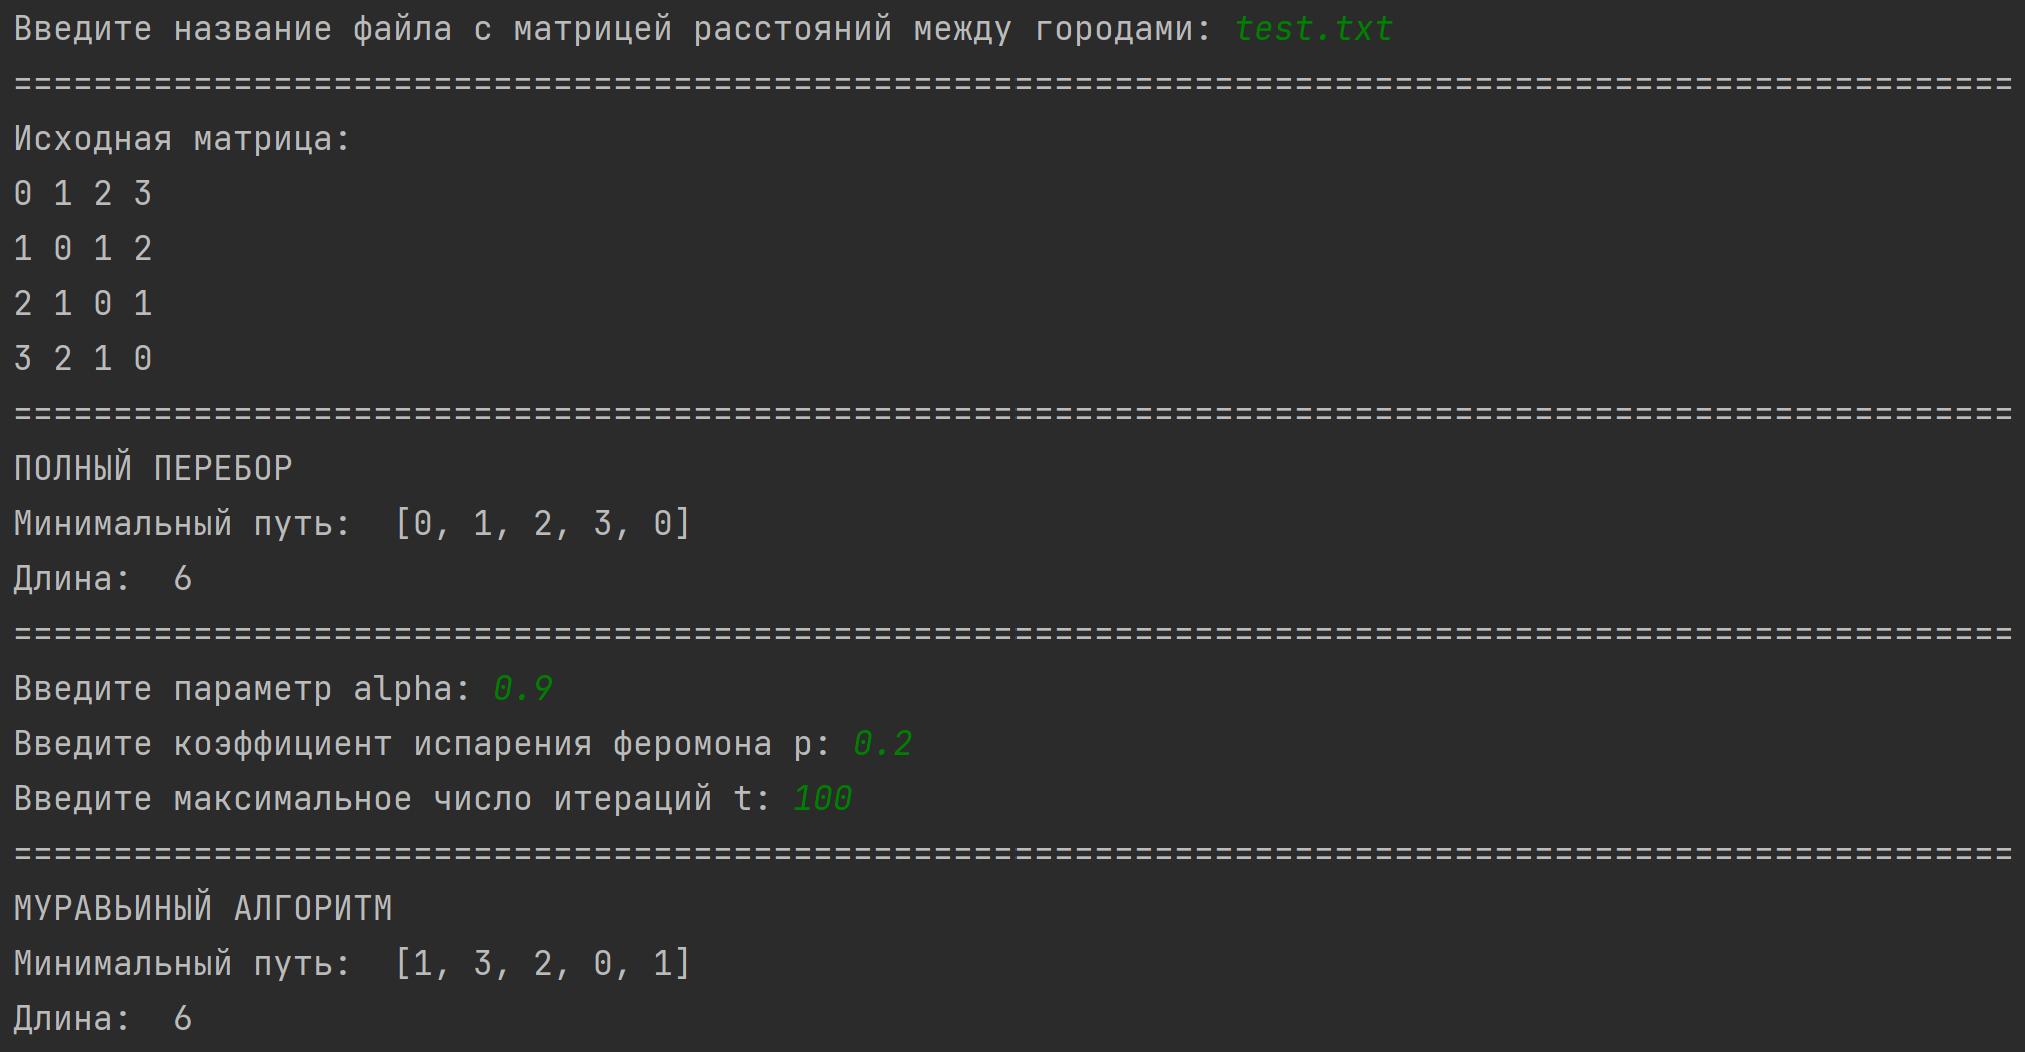
\includegraphics[width=420pt]{inc/output.png}
	\caption{Пример работы реализаций алгоритмов}
	\label{fig:output}	
\end{figure}

\vspace{\baselineskip}
\subsection{Сравнение трудоемкостей реализаций}
\vspace{\baselineskip}

Задача коммивояжера является $NP$-трудной, и точный переборный алгоритм ее решения имеет факториальную сложность $O(n!)$. 

Сложность муравьиного алгоритма равна $O(t_{max} \cdot m \cdot n^2)$, то есть она зависит от времени жизни колонии, количества городов и количества муравьев в колонии~\cite{ulyanov}. 
В разработанной реализации количество муравьев равно количеству городов, и трудоемкость муравьиного алгоритма равна $O(t_{max} \cdot n^3)$.

\vspace{\baselineskip}
\subsection{Сравнение времени выполнения реализаций алгоритмов}
\vspace{\baselineskip}

Измеряется время работы реализаций алгоритмов в зависимости от размера матрицы. 
Параметры для муравьиного алгоритма следующие: $\alpha = 1$; $p = 0.5$; $t\_max = 1000$.

На рисунке \ref{fig:research} приведены результаты сравнения времени выполнения реализаций алгоритмов.
\clearpage

\begin{figure}[h!btp]
	\centering
	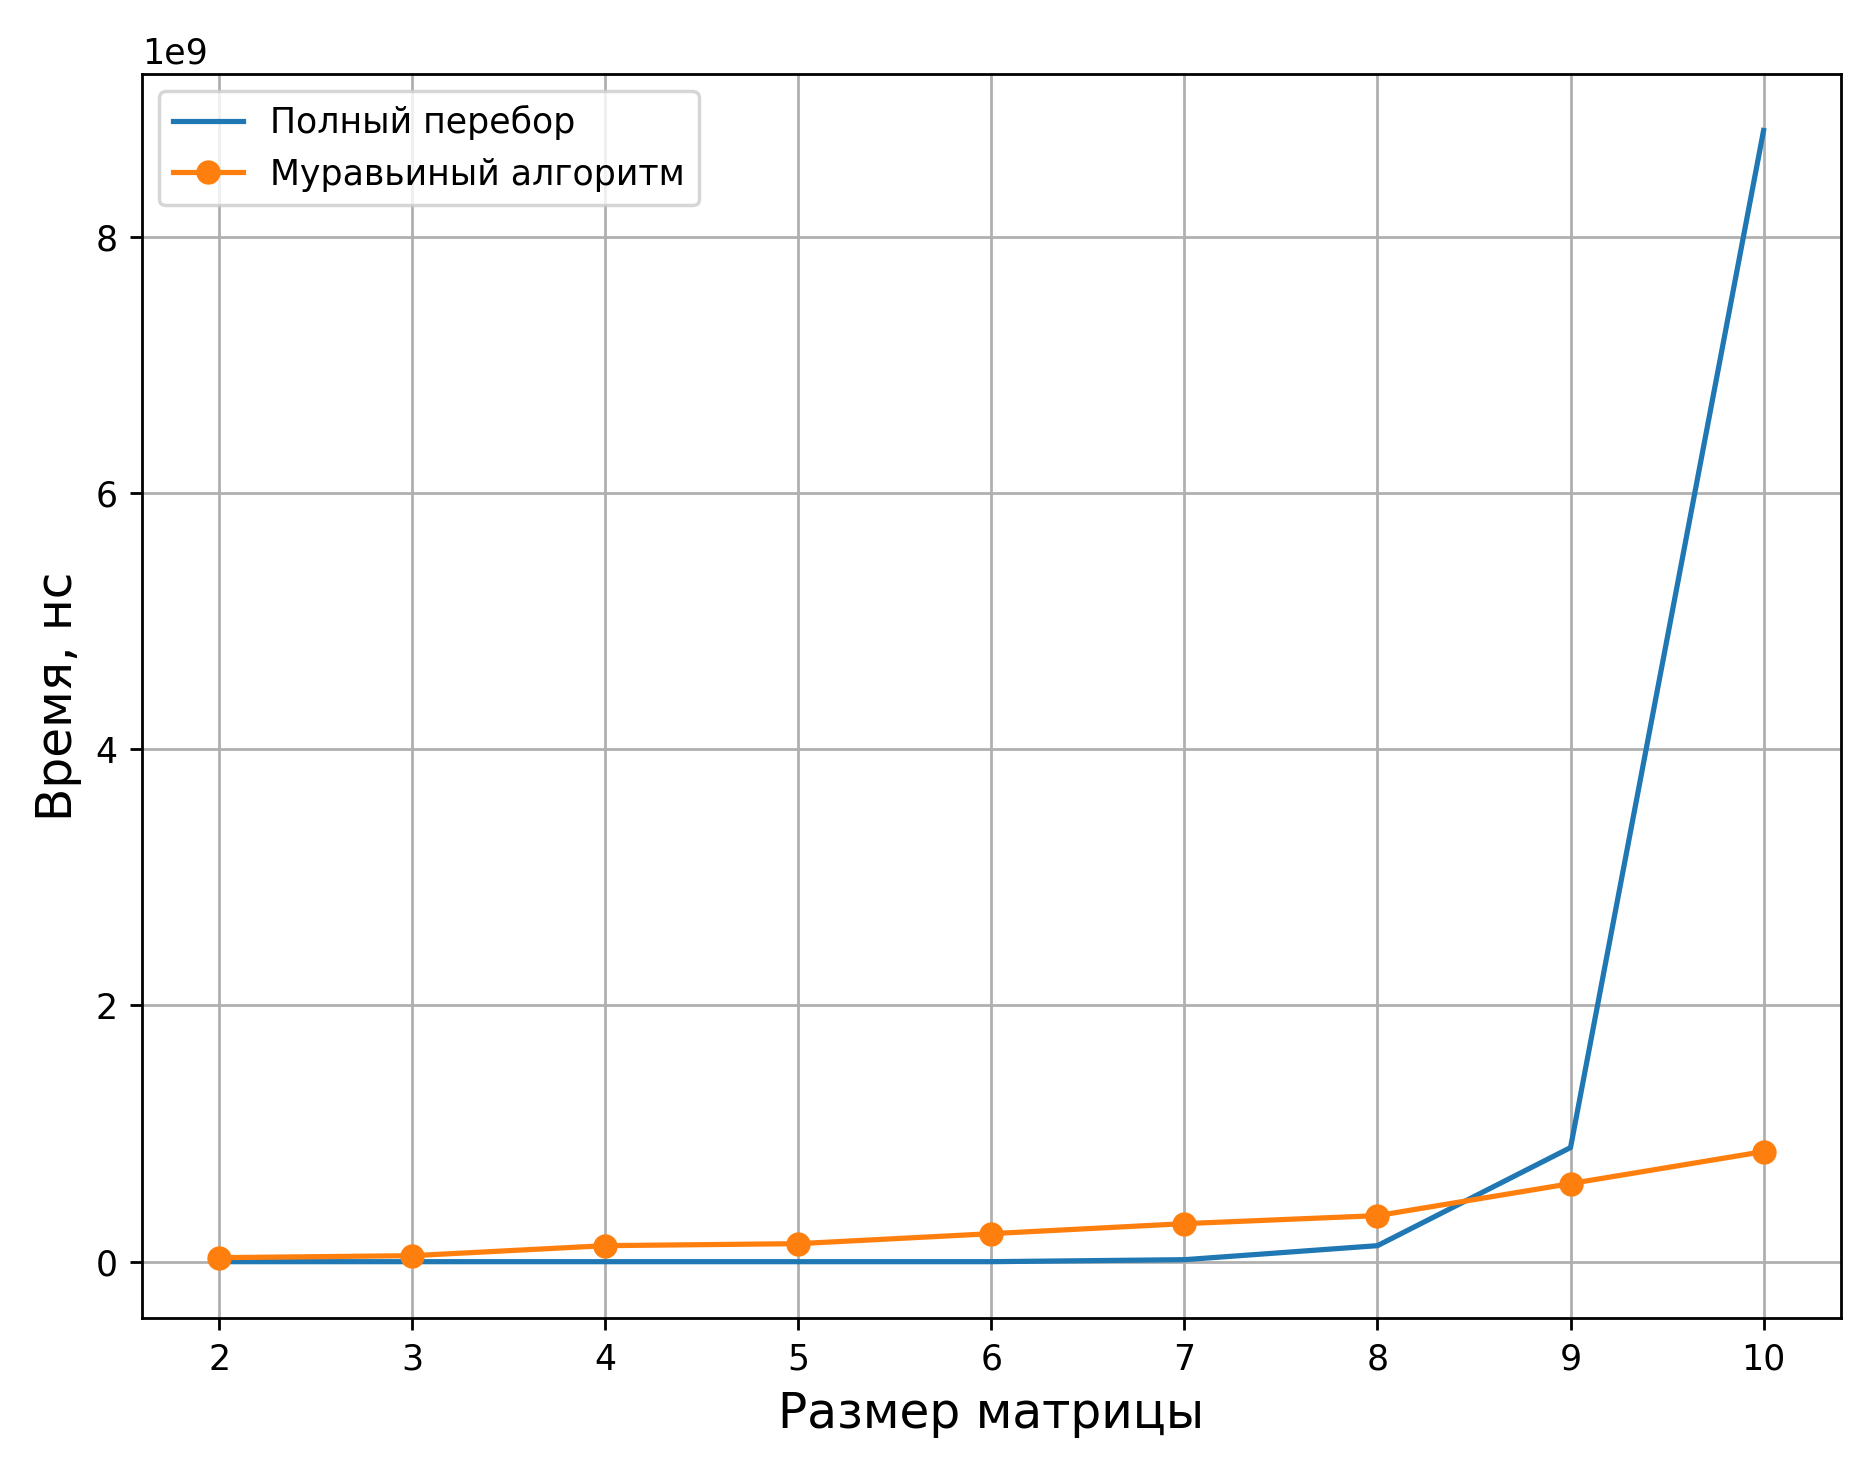
\includegraphics[width=400pt]{inc/time.png}
	\caption{Зависимость времени работы реализаций от размера матрицы расстояний}
	\label{fig:research}	
\end{figure}

\subsection{Параметризация муравьиного алгоритма}
\vspace{\baselineskip}

В муравьином алгоритме вычисления проводятся с использованием таких настраиваемых параметров, как $\alpha$ --- коэффициент жадности, $p$ --- коэффициент испарения феромона, $t_{max}$ --- время жизни колонии,  количество итераций. 
Параметризация алгоритма подразумевает подбор таких параметров, при которых алгоритм находит решение, наиболее близкое к эталонному --- найденному с помощью полного перебора. 

Параметризация проводится на двух классах данных: в первом (small) разброс длин путей равен 10, во втором (large) --- 1000. 
 
Рассматриваются матрицы размерности 11 × 11. 
Для параметров  $\alpha$ и $p$ независимо друг от друга задаются значения [0.1, 0.25, 0.5, 0.75, 0.9], а для $t\_max$ --- [100, 200, 300, 400, 500]. 

Результаты параметризации приведены в таблице \ref{tbl:param} приложения A, где $diff\_x$ --- разница между эталонным решением и решением, полученным с помощью муравьиного алгоритма на классе данных $x$.

Результаты параметризации в зависимости от количества итераций приведены в таблице \ref{tabular:iter_num}.

\begin{table}[h!]
	\begin{center}
	    \begin{threeparttable}
	    \captionsetup{justification=raggedright, singlelinecheck=off}
	    \caption{\label{tabular:iter_num} Зависимость точности от количества итераций}
		\begin{tabular}{|>{\centering}p{0.3\linewidth}|>{\centering}p{0.1\linewidth}|p{0.1\linewidth}<{\centering}|p{0.1\linewidth}<{\centering}|p{0.1\linewidth}<{\centering}|}
			\hline
			\multirow{2}*{Количество итераций} & \multicolumn{2}{c|}{Количество ошибок} & \multicolumn{2}{c|}{Средняя ошибка} \\
                \cline{2-5}
                & small & large & small & large \\
                \hline
			100 & 13 & 13 & 1.20 & 123.04 \\
                \hline
                200 & 11 & 9 & 0.84 & 87.04 \\
                \hline
                300 & 7 & 6 & 0.56 & 48.48 \\
                \hline
                400 & 6 & 8 & 0.32 & 48.44 \\
                \hline
                500 & 2 & 1 & 0.08 & 6.92 \\
                \hline
		\end{tabular}
		\end{threeparttable}
	\end{center}
\end{table}

С ростом количества итераций количество ошибок и средняя ошибка падают для обоих классов данных. 

От значений $\alpha$ и $p$ зависимостей не обнаружено, что говорит о том, что значения параметров должны регулироваться для каждой конкретной задачи. 
Лучшие параметры --- это параметры, при которых значения ошибок минимальны для обоих классов данных. 
Например, в рассматриваемом случае лучшими комбинациями аргументов на количестве итераций 100 являются (0.5, 0.1), (0.5, 0.75), (0.75, 0.25), (0.9, >0.1), где первое значение --- $\alpha$, а второе --- $p$.

\vspace{\baselineskip}
\subsection*{Вывод}
\vspace{\baselineskip}

Применимость алгоритмов зависит от того, насколько велик размер матрицы расстояний.
При размерах $N < 9$ реализация алгоритма полного перебора работает быстрее, чем реализация муравьиного алгоритма: например, при $N = 8$ --- в 4 раза.
Но при дальнейшем увеличении размера матрицы реализация муравьиного алгоритма начинает выигрывать по времени. Так, при $N = 10$ реализация муравьиного алгоритма превосходит реализацию перебора в 13 раз.

Заранее проведенная параметризация может помочь настроить муравьиный алгоритм так, что и он будет в большинстве случаев выдавать точный ответ, несмотря на то, что алгоритм предназначен для приближенного решения задачи коммивояжера.
